%=======================================================================
%
% ------------------------------------------------------------------------
% ------------------------------------------------------------------------
% abnTeX2: Modelo de Trabalho Academico  em conformidade com 
% ABNT NBR 14724:2011: Informacao e documentacao - Trabalhos academicos
% ------------------------------------------------------------------------
%Customização Unoesc
% ------------------------------------------------------------------------
% Autor:  Jonas Alessi(alessi.jonas@gmail.com
% Versão: 10 de Julho 2013.
% Edição: TexStudio
% Codificação: UTF-8
% LaTeX:  abnTeX2
%
%=======================================================================

\documentclass[
	% -- opções da classe memoir --
	12pt,				% tamanho da fonte	
	oneside,          % não imprimir em verso e anverso, oposto do twoside 
	a4paper,			% tamanho do papel. 
	% -- opções da classe abntex2 --
	chapter=TITLE,		% títulos de capítulos convertidos em letras maiúsculas
	section=TITLE,		% títulos de seções convertidos em letras maiúsculas
	subsection=TITLE,	% títulos de subseções convertidos em letras maiúsculas
	%subsubsection=TITLE,% títulos de subsubseções convertidos em letras maiúsculas
	% -- opções do pacote babel --
	english,			% idioma adicional para hifenização
	brazil			% o último idioma é o principal do documento
	,sumario=tradicional,
	]{abntex2-unoesc}


% ---
% Pacotes fundamentais 
% ---
\usepackage{cmap}				% Mapear caracteres especiais no PDF
\usepackage{times}			    % Usa a fonte Latin Modern			
\usepackage[T1]{fontenc}		% Selecao de codigos de fonte.
\usepackage[utf8]{inputenc}		% Codificacao do documento (conversão automática dos acentos)
\usepackage{lastpage}			% Usado pela Ficha catalográfica
\usepackage{indentfirst}		% Indenta o primeiro parágrafo de cada seção.
\usepackage{color}				% Controle das cores
\usepackage{graphicx}			% Inclusão de gráficos
\usepackage{amsfonts}			% Símbolos
%----Ajuste no alinhamento das listas
\usepackage{enumitem}
\setitemize[0]{itemindent=0.4cm,itemsep=0pt}
\setenumerate[0]{itemindent=0.5cm,itemsep=0pt}
%------
% ---
% Pacotes de citações
% ---
\usepackage[brazilian,hyperpageref]{backref}	 					  % Paginas com as citações na bibl
\usepackage{fancyhdr}
\usepackage[a4paper]{geometry}
%Referência
\usepackage[alf, 	
			 		abnt-emphasize=bf,
				    abnt-url-package=none,
				    abnt-repeated-title-omit=yes,
				    abnt-full-initials=yes,                                        %yes nome por extenso, no apenas iniciais
					abnt-etal-list=3												%abreviar com mais de 3 autores
]{abntex2/abntex2cite}				 														    % Citações padrão ABNT
\usepackage{lipsum}							   								       % para geração de dummy text

%\captionsetup[table]{justification=raggedright}
% Configurações de aparência do PDF final
% alterando o aspecto da cor azul
\definecolor{blue}{RGB}{41,5,195}

% --- 
% Espaçamentos entre linhas e parágrafos 
% --- 
% O tamanho do parágrafo é dado por:
\setlength{\parindent}{1.25cm}
\linespread{1.5}

%Espaçamento depois dos títulos
\setlength{\afterchapskip}{\baselineskip}
% %\setlength{\afterchapskip}{\lineskip}

% Controle do espaçamento entre um parágrafo e outro:
\setlength{\parskip}{0cm}  % tente também \onelineskip

\hangcaption
\captionstyle[\raggedright]{}

%Estava mostrando nas referencias quais paginas estavam sendo referenciadas
\renewcommand{\backref}{}
\renewcommand*{\backrefalt}[4]{}

%Reduzir a fonte do caption
%\captionnamefont{\centering\ABNTEXfontereduzida}
%\captiontitlefont{\centering\ABNTEXfontereduzida}
%Ajuste nas listas de tabela, ilustrações e quadros
\setlength\cftbeforechapterskip{0pt}
% ---
% compila o indice
% ---
\makeindex
% ---

%----Include da capa é fora do documento 
% ---
% Informações de dados para CAPA e FOLHA DE ROSTO
% ---

\titulo{\textbf{Um modelo algorítmico para previsão do mercado acionário}}
\autor{\textbf{JEAN CARLO CORSO}}
\local{Videira - SC}
\data{2018}
\orientador[Orientador:]{Wanderson Rigo}
\coorientador{Tiago Heineck}
%\supervisor{Supervisor}  % no caso de ser estágio
\instituicao{ Ministério da Educação\\
        Secretaria de Educação Profissional e Tecnológica\\
        Instituto Federal Catarinense\\\vspace{-0.2cm}
        Câmpus Videira}
\tipotrabalho{Trabalho de Conclusão de Curso}
% O preambulo deve conter o tipo do trabalho, o objetivo, 
% o nome da instituição e a área de concentração 
\preambulo{Trabalho de Conclusão de Curso apresentado ao
Curso de graduação em Ciência da Computação do
Instituto Federal de Educação Ciência e
Tecnologia Catarinense – Câmpus Videira para
obtenção do título de bacharel em Ciência da Computação

Orientador(a): Wanderson Rigo

Coorientador(a): Tiago Heineck}
% ---


%---

\begin{document}
% Retira espaço extra obsoleto entre as frases.
\frenchspacing 

% ----------------------------------------------------------
% ELEMENTOS PRÉ-TEXTUAIS
% ----------------------------------------------------------

%--- CAPA ----
\imprimircapa

% --- FOLHA DE ROSTO
\imprimirfolhaderosto
% \imprimirfolhaderosto* (o * indica que haverá a ficha bibliográfica)

% Inserir FOLHA DE APROVAÇÃO
\begin{folhadeaprovacao}

  \begin{center}
  \vspace*{-1.2cm}
    {\large\imprimirautor}

    \vspace*{\fill}\vspace*{\fill}\vspace*{\fill}
    {\large\imprimirtitulo}
    \vspace*{\fill}\vspace*{\fill}
    
    \hspace{.45\textwidth}
    \begin{minipage}{.5\textwidth}
        \imprimirpreambulo
    \end{minipage}%
    \vspace*{\fill}
   \end{center}
    
  \begin{center}
  	 Videira (SC), 21 de Maio de 2018 
  \end{center}
  

    \vspace{-1cm}

  
   \assinatura{\begin{center}\vspace{-0.7cm}\imprimirorientador \\ 
   					   Instituto Federal de Educação Ciência e Tecnologia Catarinense – Campus Videira
   					   \end{center}
   					    
   } 
    \assinatura{\begin{center}\vspace{-0.7cm}\imprimircoorientador \\ 
   					   Instituto Federal de Educação Ciência e Tecnologia Catarinense – Campus Videira
   					     \end{center}
   }
    \begin{center}
  	\textbf{ BANCA EXAMINADORA }
   \end{center}
   \vspace{-1cm}

    \assinatura{\begin{center}\vspace{-0.7cm}Mauricio Natanael Ferreira \\ 
   					    Instituto Federal de Educação Ciência e Tecnologia Catarinense – Campus Videira
   					    \end{center}
    }
     \assinatura{\begin{center}\vspace{-0.7cm}Manasses Ribeiro \\ 
   					    Instituto Federal de Educação Ciência e Tecnologia Catarinense – Campus Videira
   					    \end{center}
    }
    

    \vspace*{1cm}
  
\end{folhadeaprovacao}

% DEDICATÓRIA
%\begin{dedicatoria}
 \vspace*{\fill}
 \noindent
  \raggedleft
 \begin{minipage}{.54\textwidth}
    Dedico este trabalho a meus pais, fonte de meus conhecimentos  e saber. Graças a eles, tornei-me uma pessoa capaz de lutar para que meus sonhos e objetivos fossem sempre alcançados, sem jamais desanimar. Considero-me forte porque eles me ensinaram a ser forte.
   \end{minipage}
\end{dedicatoria}


% AGRADECIMENTO
%\begin{agradecimentos}

\lipsum[1-1]


\end{agradecimentos}

%EPÍGRAFE
%\begin{epigrafe}
    \vspace*{\fill}
	\begin{flushright}
		Não vos amoldeis às estruturas deste mundo, \\
		mas transformai-vos pela renovação da mente, \\
		a fim de distinguir qual é a vontade de Deus: \\
		o que é bom, o que Lhe é agradável, o que é perfeito.\\
		(Bíblia Sagrada, Romanos 12, 2)
	\end{flushright}
\end{epigrafe}

% RESUMO

% resumo em português
\begin{resumo}
\noindent
Empresas de capital aberto são valoradas no mercado pelo valor dado à suas ações. A previsão do valor de uma determinada ação do mercado acionário é um assunto que está sendo muito discutido nos últimos anos, porém ainda não se tem um método eficaz para a previsão exata do valor de tal ação. Este trabalho propõe o uso de uma rede neural na previsão do valor de ações visando munir o acionista com informações de boa precisão na hora da tomada de decisão sobre investimento no mercado acionário. Para a validação e comprovação da eficiência da rede serão realizadas testes com dados históricos reais da bolsa de valores. 


 \vspace{0.2cm}
    
 
 Palavras-chave: Redes neurais artificiais. Previsão. Mercados de ações. Séries temporais.
\end{resumo}

% resumo em inglês
\begin{resumo}[Abstract]	
 	\begin{otherlanguage*}{english}
 	\noindent 
	\textit{
	Public companies are valued in the market by the value given to their shares. The prediction of the value of a particular stock market share is a subject that has been much discussed in recent years, but there is still no effective method for accurately predicting the value of such stock. This work proposes the use of a neural network in predicting the value of shares aiming to provide the shareholder with accurate information at the time of decision on investment in the stock market. For the validation and verification of the efficiency of the network tests will be carried out with historical historical data of the stock exchange.
	} 
   \vspace{0.2cm}
 
   
    Key-words: Artificial neural networks. Prediction. Stock markets. Time series.
 	\end{otherlanguage*}
\end{resumo}

% lista de ilustrações
\pdfbookmark[0]{\listfigurename}{lof}
\listoffigures*
\cleardoublepage
% ---

% lista de quadros
% --- 
%PRECISO VER COMO FAZER O CONTROLE DE QUANDO TIVER MENOS Q 10 VAI PARA LISTA DE ILUSTRAÇÕES
%\pdfbookmark[0]{\listofquadrosname}{loq}
%\listofquadros*
%\cleardoublepage
% ---

% LISTA DE TABELAS
\pdfbookmark[0]{\listtablename}{lot}
\listoftables*
\cleardoublepage  %-- força proxima pagina

% ---
% inserir lista de abreviaturas e siglas
% ---
\begin{siglas}
  \item[AI] \textit{Artificial Intelligence} (Inteligência Artificial)
  \item[RNA] Rede Neural Artificial
\end{siglas}
% ---

% ---
% inserir lista de símbolos
% ---
%\begin{simbolos}
%  \item[$ \Gamma $] Descrever o que o símbolo representa em seu trabalho. Exemplo abaixo.
%  \item[$ \omega $] Frequência angular [rad/s].
%  \item[$ \zeta $] Coeficiente de amortecimento.
%\end{simbolos}
% ---

% SUMARIO
\pdfbookmark[0]{\contentsname}{toc}
\tableofcontents*
\cleardoublepage

% ------------------------------------------------------
% ELEMENTOS TEXTUAIS
% ------------------------------------------------------
\textual
% INTRODUÇÃO
% ----------------------------------------------------------
% Introdução
%Ex: \chapter{TÍTULO A SER IMPRESSO NO CORPO DO TEXTO}{Título no cabeçalho}{Título no Sumario}
% ----------------------------------------------------------
\chapter{INTRODUÇÃO} 

	Uma ação é a menor parcela do capital social de uma empresa ou sociedade anônima. Cada uma delas representam pequenas fatias do capital de uma determinada empresa, e o seu valor varia constantemente influenciado por vários fatores, entre eles pode-se destacar a lei da oferta e da procura (o quanto investidores procuram uma determinada ação para comprar), a situação política e econômica de cada país, pela administração da empresa entre outras inúmeras variáveis \cite{REPORTERBRASIL}. Sendo assim, isto interfere nos preços de uma ação, tornando-se muito difícil prever com exatidão o valor que uma ação terá ao final do pregão.
	
	Mesmo com todos os riscos e a alta volatilidade do mercado acionário, existem pessoas que dedicam suas vidas a analisar gráficos e tentar prever o comportamento das ações, que em uma primeira impressão parece ser aleatório, mas por mais experiente que o investidor seja é muito difícil alguém analisar por si só qual é a tendência de uma ação, pois para analisar a tendência de uma certa ação o investidor deve levar em consideração uma série de fatores como por exemplo as altas e baixas anteriores, volume de ações negociados, o valor de mercado de uma empresa, a liquidez corrente (ativos circulantes divididos pelos passivos circulantes) e o retorno do patrimônio líquido (ROE). Agora imagine uma análise de todos esses itens em 100, 200 ou 1000 empresas diferentes, fazer uma análise sobre estas condições é muito cansativo, e ainda dependeria-se de fatores psicológicos do investidor \cite{FOGACA}.   
	
	Uma boa alternativa para alcançar um valor aproximado da variação do preço de uma determinada ação é através do uso de redes neurais para fazer a análise de séries temporais \cite{GIACOMELL}.  
	
	O estudo de redes neurais para previsão de séries temporais cresceu muito ao longo dos últimos anos. O principal fator para a escolha de redes neurais na resolução deste tipo de problema é devido ao seu bom comportamento na solução de problemas não lineares que contêm muitas variáveis \cite{GIACOMELL}, como é o caso do mercado acionário que possui vários fatores que podem interferir no preço das ações. Considerando  a dificuldade em prever a variação dos preços de uma ação, dada a quantidade de variáveis que interferem na mesma, têm-se um crescente aumento no interesse em investimentos na automatização/previsão de operações, sendo estas as mais confiáveis quanto possível.    
	
	Considerando-se que os fatores que alteraram os preços de uma determinada ação continuarão afetando o seu valor no futuro, justifica-se a criação ou estudo de um método para capturar esses fatores a fim de prever quando estes eventos se repetirão.
	
	O presente trabalho propõe a criação de um algoritmo baseado em ensembles de redes neurais para analisar as séries temporais, com o intuito de identificar comportamentos parecidos e prever seus resultados tomando como base uma análise técnica, que por sua vez interpreta que todos os dados que podem ser utilizados na previsão estão contidos no valor da ação. Este tipo de análise também afirma que as variações do passado tendem a se repetir no futuro\cite{GIACOMELL}. Desta forma pretende-se alcançar maiores lucros nos investimentos, pois quando o investidor passa a responsabilidade da análise para uma máquina elimina-se o fator emocional do investidor possibilitando uma análise soberana. 

\section{OBJETIVOS}
Esta seção contém os objetivos do trabalho, que estão divididos em duas sub categorias, gerais e específicos.

\subsection{Objetivo geral}
Elaborar e calibrar uma rede neural artificial de modo que,  através da análise de séries temporais, ela seja capaz de projetar com acurácia variações dos valores de ações.

\subsection{Objetivos específicos}

 \begin{itemize}
	\item Montar uma base de dados históricos de transações do mercado acionário e identificar os melhores critérios que podem ser utilizados na elaboração da rede.
	\item Montar uma base de testes para avaliar a acurácia da rede.
\end{itemize}

\section{Metodologia}
As seções a seguir tem por objetivo informar como o trabalho será realizado.

\subsection{Levantamento Bibliográfico}
Primeiramente será realizado um estudo em livros, artigos e algumas páginas web, para maior compreensão das tecnologias de redes neurais existentes, compreender seu funcionamento e também identificar o que já está sendo usado. 

\subsection{Sistemática}
Inicialmente, serão coletados dados históricos acerca da variação dos preços de ações em várias empresas, os dados serão extraídos da plataforma Yahoo Finances no formato CSV. Em seguida, será realizado um estudo mais aprofundado com o intuito de identificar as causas destas variações, e os dados que podem ser usados para a previsão. 

Em seguida captura e estudo dos dados, será elaborada uma rede neural, as funções de ativação que melhor se adaptem ao problema e a escolha de um algoritmo de aprendizado.

Logo após a definição da rede neural será iniciado o treinamento da rede neural, com os dados históricos obtidos no processo anterior. Com a rede neural já calibrada, será iniciado os testes de eficiência, a fim de verificar e comprovar sua eficiência.

Para a realização dos testes será comparada a saída da rede neural com os valores reais da ação no período de tempo analisado. Estes dados também serão usados para um retreinamento da rede neural.



%FUNDAMENTAÇÃO TEÓRICA
\chapter{REFERENCIAL TEÓRICO }

\section{Mercado Financeiro}
Muitos conceitos que serão utilizados neste trabalho são referentes ao mercado financeiro, portanto para sintonizar os leitores, nesta secção será apresentada uma breve descrição dos conceitos referentes ao mercado financeiro.

\subsection{Bolsa de valores}
A bolsa de valores é um ponto comum onde as empresas podem negociar suas ações. Todos os países que possuem empresas de capital aberto possuem uma bolsa de valores, no Brasil este ponto de compra e venda de ações é chamado de Bovespa. A Bovespa é a única regulamentada no Brasil\cite{EQUIPETORORADAR}. Abaixo na Figura 1 pode-se ver as principais bolsas de valores até o momento.

 \begin{figure}[htb]
 \centering
 	\caption{Principais bolsas de valores}
 	\label{fig:principais-bolsas}
 	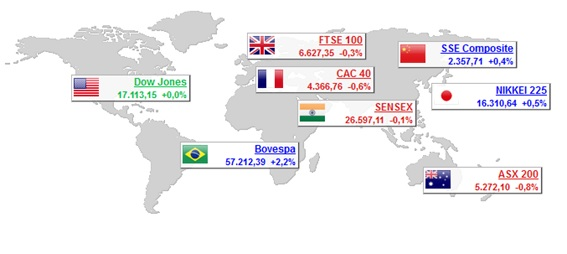
\includegraphics[scale=0.8]{figuras/principais-bolsas.jpg}
 	\fonte{https://br.advfn.com/mundo}
 \end{figure}
 
 A Figura 1 acima também indica o índice de cada bolsa de valores ali representada. O índice da bolsa é dado pelo desempenho de compra e venda de ações negociadas dentro da bolsa em questão, e indica o desempenho médio do mercado acionário de cada país\cite{IBOVESPA}.

\subsection{Preços}
Geralmente a forma mais comum de se analisar o desempenho dos preços de uma ação é o valor de fechamento, esta é a forma que a mídia usa para fazer a divulgação, porém existem muitas variações do preço da ação ao longo do dia. Para se estabelecer um preço para uma determinada ação baseia-se a lei da oferta e da procura, quanto mais compras uma determinada ação ter maior será seu valor, também pode ser usado como métrica a perspectiva de crescimento da empresa\cite{CITI}.  Quando se busca os dados históricos acerca dos preços de uma ação será encontrado estes dados usando diferentes métricas, o site da Bovespa e do yahoo finance disponibilizam as seguintes métricas:

 \begin{itemize}
	\item Abertura - É o valor da ação no momento da abertura do pregão.
    \item Máximo - Indica o valor mais alto que a ação atingiu durante o dia. Esta é uma métrica muito interessante para saber qual é a tendência da ação, pois se o valor máximo for muito maior que o valor de fechamento indica que houve queda no preço da ação e a tendência é que continue caindo. Se o valor máximo for muito próximo do valor de fechamento indica uma tendência de alta.
    \item Mínimo - Indica o menor valor que a ação teve no período. A interpretação é ao máximo.
    Fechamento - Indica o valor da ação no final do pregão. É a métrica mais comumente utilizada pela mídia para a divulgação dos preços de ações.
    \item Fechamento Ajustado - É o valor de fechamento após o cálculo e distribuição dos dividendos.
    \item Volume - Indica quantas ações foram negociadas no período.
\end{itemize}

\section{Série Temporal}
“A classe de fenômenos cujo processo observacional e consequente quantificação numérica gera uma sequencia de dados distribuídos no tempo é denominada série temporal” \cite{MUELLER}, portanto uma série temporal é a variação de um valor ao longo do tempo. Este valor pode variar apenas em função do tempo eu em função de um conjunto de variáveis, desde que seja em função do tempo\cite{AMADOR}, ou como \citeonline[]{PEDROSO} define série Temporal é uma realização ou trajetória de um processo estocástico. Pode-se citar como exemplo de séries temporais as temperaturas máximas e mínimas diária da cidade de Videira, a variação do preço do dólar ou a variação do preço de uma ação. Abaixo na Figura 2 temos uma representação de uma série temporal das ações de uma empresa qualquer.

\begin{figure}[htb]
 \centering
 	\caption{Série temporal}
 	\label{fig:Série temporal}
 	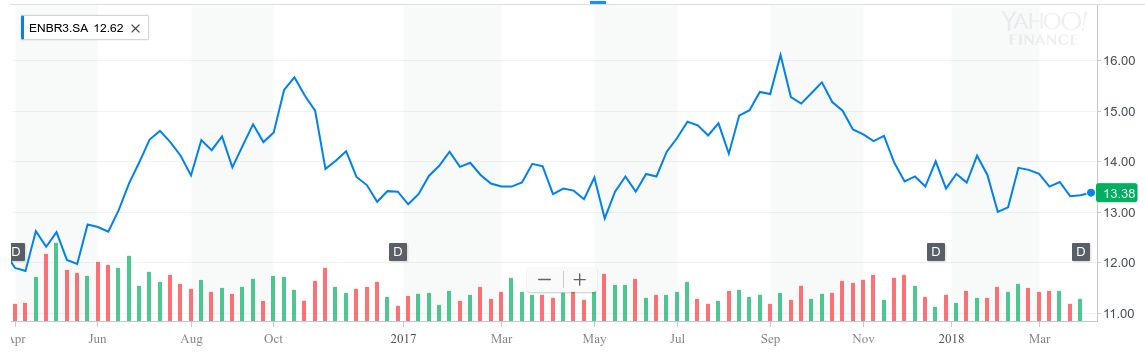
\includegraphics[scale=0.5]{figuras/serie-temporal-yahoo.png}
 	\fonte{Adaptada de https://finance.yahoo.com}
 \end{figure}

Na Figura 2 pode-se perceber que os valores da ação desta empresa tendem a ter valores próximos em determinados meses do ano. As variações sempre seguem um padrão, e com o uso de redes neurais artificiais pode-se identificar este padrão e tentar chegar em um valor aproximado da ação.

\section{Inteligência Artificial}
Desde os primórdios da humanidade nós tentamos compreender o que é a inteligência humana, como que um mero humano, que nada mais é que um simples pedaço de matéria, consegue compreender e modificar um universo muito maior. O campo da inteligência artificial ou IA, tenta compreender e reproduzir a inteligência humana em máquinas \cite{RUSSUEL}. 

A IA é um campo relativamente novo, os trabalhos relacionados ao desenvolvimento desta ciência começaram logo após a segunda guerra mundial e o nome desta nova subárea da ciência foi criado em meados de 1956.

Para definir Inteligência artificial é necessário quebrar o termo, dessa forma teremos os termos “Inteligência” e “Artificial”, desta forma podemos dizer que “artificial” é tudo aquilo feito pelo homem \cite{ROSA}. Para definir o termo “inteligência” é um pouco mais difícil, para isso precisamos recorrer a filosofia e psicologia, se olharmos no dicionário inteligência é a capacidade de compreender e resolver novos problemas e conflitos e de adaptar-se a novas situações. Uma boa definição para IA é, segundo Winston (1992), “O estudo de computações que tornem possível perceber e agir”.

\subsection{Redes Neurais Artificiais}
As redes neurais artificiais (RNA’s) são sistemas paralelos distribuídos compostos por unidades de processamento simples (neurônios artificiais) que calculam determinadas funções matemáticas, seu objetivo é imitar o comportamento do cérebro biológico, porém possuem um número muito inferior de neurônios, estes neurônios podem processar inúmeras variáveis ao mesmo tempo. O grande diferencial das RNA’s para outros sistemas é a capacidade de interpretar o meio externo e se adaptar a ele \cite{FINOCCHIO} \cite{BRAGA}.

\subsubsection{Neurônio artificial}
O neurônio artificial é uma estrutura muito simples inspirada no neurônio biológico. Da mesma forma que um neurônio biológico tem os dendritos responsáveis por receber os impulsos elétricos e conduzi-los até o corpo celular e o axônio encarregado de enviar a saída até o dendrito do próximo neurônio (Figura 3), o neurônio artificial é composto por várias entradas (dendritos) que recebem os valores x1, x2, x3, …, xn correspondentes as ativações dos neurônios anteriores, possui também um terminal de saída y que representa o axônio do neurônio biológico. Cada entrada entrada do neurônio artificial possui um peso, chamado de peso sináptico, dado por w, os pesos servem para o neurônio artificial identificar o grau de relevância daquela entrada \cite{BRAGA}. O neurônio artificial está representado na Figura 4.

\begin{figure}[htb]
 \centering
 	\caption{Neurônio Biológico}
 	\label{fig:Neurônio Biológico}
 	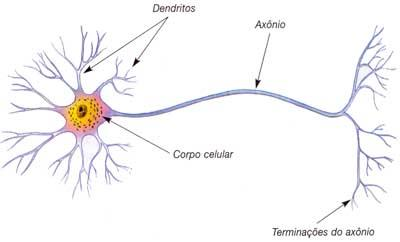
\includegraphics[scale=1.8]{figuras/neuronio-biologico.jpg}
 	\fonte{www.researchgate.net}
 \end{figure}
 
\begin{figure}[htb]
 \centering
 	\caption{Neurônio Artificial}
 	\label{fig:Neurônio Artificial}
 	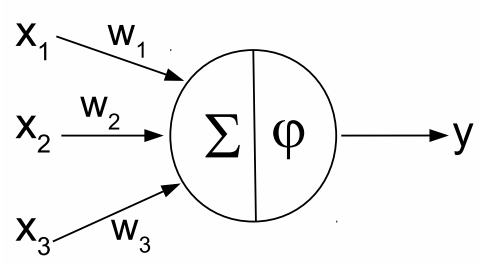
\includegraphics[scale=0.9]{figuras/neuronio-artificial.png}
 	\fonte{\cite{GIACOMELL}.}
 \end{figure}
 
 \subsubsection{Função de ativação}
 A função de ativação é responsável por gerar a saída do neurônio a partir da somatória das entradas com seus respectivos pesos. Esta função tem efeito apenas no neurônio em que ela está empregada.

As funções de ativação mais comumente utilizadas são: função logística e função tangente hiperbólica. A função logística ou sigmóide é dada por:

$${\sigma(x) = {1\over 1+e^x}}$$

Esta função de ativação foi amplamente utilizada em RNAs por ser mais parecido com a biologia pois como neurônios biológicos funcionam de forma binária, a função sigmóide é uma boa forma de modelar esse comportamento, já que assume valores apenas entre 0 e 1 \cite{FACURE}.

Similar a função sigmóide a função tangente hiperbólica varia de -1 a 1. \citeonline[]{FACURE} diz que por se aproximar mais da identidade a função tangente hiperbólica é melhor do que a sigmóide para as camadas ocultas. A função tangente hiperbólica é dada por:

 $${{tanh(x) = 2\sigma(2x)-1}}$$
 $${{{tanh^'}(x) = 1-{tanh^2}(x)}}$$
 
 \subsubsection{RNA Feedforward}
 Também chamada de acíclica, neste tipo de rede todas as saídas dos neurônios estão direcionados para as entradas dos neurônios da próxima camada, a saída de um neurônio deve servir de entrada para todos os neurônios da camada superior e não é permitido o retorno da informação, desta forma a rede segue em apenas um sentido, sempre para frente, como mostra a Figura 5. Este tipo de rede é bastante utilizado em problemas não lineares para a classificação e reconhecimento de padrões \cite{INTRODUCAO}.

Para que este estilo de RNA resolva um problema deve-se fornecer os dados para os neurônios de primeira camada, e desta forma os dados serão processados e enviados para as próximas camadas até chegar a camada de saída com o resultado obtido \cite{GIACOMELL}.

\begin{figure}[htb]
 \centering
 	\caption{RNA Feedforward}
 	\label{fig:RNA Feedforward}
 	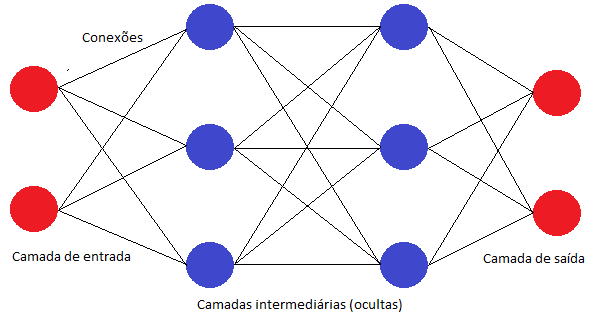
\includegraphics[scale=0.9]{figuras/rede-feedforward.png}
 	\fonte{Autor.}
 \end{figure}
 
 \subsubsection{Backpropagation}
 O backpropagation é um algoritmo de aprendizado supervisionado. Para se implementar esta técnica é necessário a existência de um “professor” que será responsável por estimular as entradas da rede  e comparar as saídas da mesma com o resultado esperado \cite{BRAGA}, veja a Figura 6. O processo se dá da seguinte forma: a rede é carregada com um conjunto de entradas, e através de uma configuração inicial de seus pesos, gera uma saída correspondente às entradas. A saída da RNA é comparada com a saída esperada e caso o erro seja superior ao limite definido pelo programador a rede reconfigura os pesos das suas sinapses, este processo se repete até que a rede obtenha uma saída satisfatória \cite{LANHELLAS}.

\begin{figure}[htb]
 \centering
 	\caption{Aprendizado supervisionado}
 	\label{fig:Aprendizado supervisionado}
 	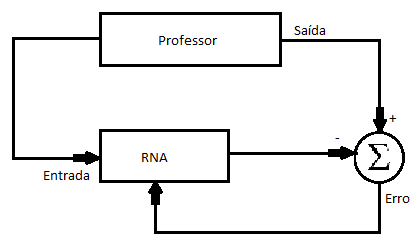
\includegraphics[scale=0.9]{figuras/aprendizado-supervizionado.png}
 	\fonte{Autor.}
 \end{figure}

% FALTA AJUSTAR \subsubsubsection{Exemplo subsubsubsection}

% TRABALHOS RELACIONADOS
\chapter{Trabalhos Relacionados}
A seção a seguir tem por objetivo apontar alguns dos trabalhos já publicados e que tenham relação com o assunto desta pesquisa. 

\section{REDES NEURAIS NA PREVISÃO DO MERCADOS FINANCEIROS}
No trabalho de \citeonline[]{BOSAIPO} ele faz testes com vários tipos de redes neurais diferentes, a que atinge melhores resultados, segundo ele, é a rede com o algoritmo de aprendizado backpropagation randomized, esta rede conta com três camadas sendo 20 neurônios na primeira 6 na segunda e 2 na última. A função de ativação usada por ele nesta rede foi a hiperbólica entre a primeira e segunda camada, e a função de ativação linear entre a segunda e a última.

Embora a rede com as configurações citadas acima tenha tido um bom resultado, há um alto índice de erros o que torna a aplicação pouco confiável. Provavelmente, como o próprio autor sugere, os erros que a rede produziu foi por causa do curto período de tempo usado para testes, o autor usou como entrada apenas as cotações e os volumes negociados nos últimos 10 dias.

Seguindo a mesma linha de raciocínio de Bosaipo \citeonline[]{OCONNOR} implementam uma rede neural que tem como dados de entrada o valor de abertura e com esses dados tenta prever se a ação terá alta ou queda ao final do dia. Esta implementação é muito boa porém não aponta qual será o valor máximo que a ação poderá atingir ao final do pregão apenas indica a tendência.

\section{USO DE ENSEMBLES DE REDES NEURAIS}
Outro trabalho bastante interessante na previsão do mercado acionário é o de \citeonline[]{GIACOMELL} que diferentemente de Bosaipo, preferiu criar e treinar uma rede que apresente ao investidor apenas a tendência do mercado, informando se os próximos movimentos serão de alta ou queda. 
Em sua pesquisa Giacomel utiliza dois ensembles de redes neurais, sendo eles específicos para cada perfil de investidor, moderado ou agressivo. No ensemble moderado o autor escolheu usar como entrada os valores de abertura, máximo, mínimo, e fechamento dos dias anteriores, com essas informações o ensemble pode produzir três saídas, alta, queda ou não sabe que representa períodos de incertezas. Este ensemble é composto por duas redes neurais e mais uma porta lógica AND que faz a junção das saídas da rede.

O ensemble agressivo é um complemento do ensemble moderado, ele usa as mesmas entradas porém possui além das duas redes neurais um indicador técnico que avalia a situação do mercado e serve de apoio na decisão. O indicador técnico usado pelo autor foi o SAR pois segundo o mesmo é o que apresentou melhor desempenho quando comparado com outros.

O autor conseguiu alcançar resultados satisfatórios com o modelo proposto, porém os lucros poderiam ser mais altos se o investidor soubesse o valor máximo e mínimo que a ação poderia alcançar no dia, pois assim saberia o momento perfeito para comprar ou vender suas ações.

\section{CONSIDERAÇÕES}
Observando as pesquisas realizadas nesta área, foi constatado que os produtos existentes utilizam apenas uma série de retornos para prever as variações futuras, o que torna o resultado inconsistente e suscetível a erros, além do mais os artigos que foram pesquisados estão preocupados em apontar apenas a tendência de uma ação, ou seja, se esta irá subir ou descer no próximo período. O presente trabalho propõe a análise de vários fatores, como o valor de abertura, o valor de fechamento do dia anterior volume negociado, valor máximo e mínimo atingido pela ação em cada período, e terá como objetivo principal apontar o valor exato(ou o mais próximo possível) dos valores futuros para que o investidor saiba o melhor momento para fazer a compra ou venda de suas ações.


% CRONOGRAMA
\chapter{Cronograma proposto}

O quadro a seguir apresenta a cronologia das atividades a serem executadas para o desenvolvimento do trabalho proposto.


% ######## init table ########
\begin{table}[h]
\caption{Cronograma}
 \centering
% distancia entre a linha e o texto
 {\renewcommand\arraystretch{1.25}
 \begin{tabular}{ l l l l l l l l l l l }
  \cline{1-1}\cline{2-2}\cline{3-3}\cline{4-4}\cline{5-5}\cline{6-6}\cline{7-7}\cline{8-8}\cline{9-9}\cline{10-10}\cline{11-11}  
    \multicolumn{1}{|p{4.283cm}|}{\textbf{Atividades} \centering } &
    \multicolumn{1}{p{0.709cm}|}{\textbf{03/18} \centering } &
    \multicolumn{1}{p{0.709cm}|}{\textbf{04/18} \centering } &
    \multicolumn{1}{p{0.709cm}|}{\textbf{05/18} \centering } &
    \multicolumn{1}{p{0.709cm}|}{\textbf{06/18} \centering } &
    \multicolumn{1}{p{0.709cm}|}{\textbf{07/18} \centering } &
    \multicolumn{1}{p{0.709cm}|}{\textbf{08/18} \centering } &
    \multicolumn{1}{p{0.709cm}|}{\textbf{09/18} \centering } &
    \multicolumn{1}{p{0.709cm}|}{\textbf{10/18} \centering } &
    \multicolumn{1}{p{0.709cm}|}{\textbf{11/18} \centering } &
    \multicolumn{1}{p{0.709cm}|}{\textbf{12/18} \centering }
  \\  
  \cline{1-1}\cline{2-2}\cline{3-3}\cline{4-4}\cline{5-5}\cline{6-6}\cline{7-7}\cline{8-8}\cline{9-9}\cline{10-10}\cline{11-11}  
    \multicolumn{1}{|p{4.283cm}|}{\textbf{Criação do plano de trabalho}} &
    \multicolumn{1}{p{0.709cm}|}{X \centering } &
    \multicolumn{1}{p{0.709cm}|}{  \centering } &
    \multicolumn{1}{p{0.709cm}|}{  \centering } &
    \multicolumn{1}{p{0.709cm}|}{  \centering } &
    \multicolumn{1}{p{0.709cm}|}{  \centering } &
    \multicolumn{1}{p{0.709cm}|}{  \centering } &
    \multicolumn{1}{p{0.709cm}|}{  \centering } &
    \multicolumn{1}{p{0.709cm}|}{  \centering } &
    \multicolumn{1}{p{0.709cm}|}{  \centering } &
    \multicolumn{1}{p{0.709cm}|}{  \centering }
  \\  
  \cline{1-1}\cline{2-2}\cline{3-3}\cline{4-4}\cline{5-5}\cline{6-6}\cline{7-7}\cline{8-8}\cline{9-9}\cline{10-10}\cline{11-11}  
    \multicolumn{1}{|p{4.283cm}|}{\textbf{Definição do PTC}} &
    \multicolumn{1}{p{0.709cm}|}{X \centering } &
    \multicolumn{1}{p{0.709cm}|}{  \centering } &
    \multicolumn{1}{p{0.709cm}|}{  \centering } &
    \multicolumn{1}{p{0.709cm}|}{  \centering } &
    \multicolumn{1}{p{0.709cm}|}{  \centering } &
    \multicolumn{1}{p{0.709cm}|}{  \centering } &
    \multicolumn{1}{p{0.709cm}|}{  \centering } &
    \multicolumn{1}{p{0.709cm}|}{  \centering } &
    \multicolumn{1}{p{0.709cm}|}{  \centering } &
    \multicolumn{1}{p{0.709cm}|}{  \centering }
  \\  
  \cline{1-1}\cline{2-2}\cline{3-3}\cline{4-4}\cline{5-5}\cline{6-6}\cline{7-7}\cline{8-8}\cline{9-9}\cline{10-10}\cline{11-11}  
    \multicolumn{1}{|p{4.283cm}|}{\textbf{Obtenção de dados}} &
    \multicolumn{1}{p{0.709cm}|}{  \centering } &
    \multicolumn{1}{p{0.709cm}|}{X \centering } &
    \multicolumn{1}{p{0.709cm}|}{X \centering } &
    \multicolumn{1}{p{0.709cm}|}{  \centering } &
    \multicolumn{1}{p{0.709cm}|}{  \centering } &
    \multicolumn{1}{p{0.709cm}|}{  \centering } &
    \multicolumn{1}{p{0.709cm}|}{  \centering } &
    \multicolumn{1}{p{0.709cm}|}{  \centering } &
    \multicolumn{1}{p{0.709cm}|}{  \centering } &
    \multicolumn{1}{p{0.709cm}|}{  \centering }
  \\  
  \cline{1-1}\cline{2-2}\cline{3-3}\cline{4-4}\cline{5-5}\cline{6-6}\cline{7-7}\cline{8-8}\cline{9-9}\cline{10-10}\cline{11-11}  
    \multicolumn{1}{|p{4.283cm}|}{\textbf{Criação do modelo computacional}} &
    \multicolumn{1}{p{0.709cm}|}{  \centering } &
    \multicolumn{1}{p{0.709cm}|}{  \centering } &
    \multicolumn{1}{p{0.709cm}|}{X \centering } &
    \multicolumn{1}{p{0.709cm}|}{X \centering } &
    \multicolumn{1}{p{0.709cm}|}{  \centering } &
    \multicolumn{1}{p{0.709cm}|}{  \centering } &
    \multicolumn{1}{p{0.709cm}|}{  \centering } &
    \multicolumn{1}{p{0.709cm}|}{  \centering } &
    \multicolumn{1}{p{0.709cm}|}{  \centering } &
    \multicolumn{1}{p{0.709cm}|}{  \centering }
  \\  
  \cline{1-1}\cline{2-2}\cline{3-3}\cline{4-4}\cline{5-5}\cline{6-6}\cline{7-7}\cline{8-8}\cline{9-9}\cline{10-10}\cline{11-11}  
    \multicolumn{1}{|p{4.283cm}|}{\textbf{Primeira implementação}} &
    \multicolumn{1}{p{0.709cm}|}{  \centering } &
    \multicolumn{1}{p{0.709cm}|}{  \centering } &
    \multicolumn{1}{p{0.709cm}|}{  \centering } &
    \multicolumn{1}{p{0.709cm}|}{X \centering } &
    \multicolumn{1}{p{0.709cm}|}{X \centering } &
    \multicolumn{1}{p{0.709cm}|}{X \centering } &
    \multicolumn{1}{p{0.709cm}|}{X \centering } &
    \multicolumn{1}{p{0.709cm}|}{  \centering } &
    \multicolumn{1}{p{0.709cm}|}{  \centering } &
    \multicolumn{1}{p{0.709cm}|}{  \centering }
  \\  
  \cline{1-1}\cline{2-2}\cline{3-3}\cline{4-4}\cline{5-5}\cline{6-6}\cline{7-7}\cline{8-8}\cline{9-9}\cline{10-10}\cline{11-11}  
    \multicolumn{1}{|p{4.283cm}|}{\textbf{Testes e ajustes da aplicação}} &
    \multicolumn{1}{p{0.709cm}|}{  \centering } &
    \multicolumn{1}{p{0.709cm}|}{  \centering } &
    \multicolumn{1}{p{0.709cm}|}{  \centering } &
    \multicolumn{1}{p{0.709cm}|}{  \centering } &
    \multicolumn{1}{p{0.709cm}|}{  \centering } &
    \multicolumn{1}{p{0.709cm}|}{  \centering } &
    \multicolumn{1}{p{0.709cm}|}{  \centering } &
    \multicolumn{1}{p{0.709cm}|}{X \centering } &
    \multicolumn{1}{p{0.709cm}|}{X \centering } &
    \multicolumn{1}{p{0.709cm}|}{X \centering }
  \\  
  \cline{1-1}\cline{2-2}\cline{3-3}\cline{4-4}\cline{5-5}\cline{6-6}\cline{7-7}\cline{8-8}\cline{9-9}\cline{10-10}\cline{11-11}  
    \multicolumn{1}{|p{4.283cm}|}{\textbf{Documentação do Projeto}} &
    \multicolumn{1}{p{0.709cm}|}{  \centering } &
    \multicolumn{1}{p{0.709cm}|}{  \centering } &
    \multicolumn{1}{p{0.709cm}|}{  \centering } &
    \multicolumn{1}{p{0.709cm}|}{  \centering } &
    \multicolumn{1}{p{0.709cm}|}{X \centering } &
    \multicolumn{1}{p{0.709cm}|}{X \centering } &
    \multicolumn{1}{p{0.709cm}|}{X \centering } &
    \multicolumn{1}{p{0.709cm}|}{X \centering } &
    \multicolumn{1}{p{0.709cm}|}{X \centering } &
    \multicolumn{1}{p{0.709cm}|}{X \centering }
  \\  
  \hline

 \end{tabular} }
 \legend{Fonte: Autor.}
\end{table}

% CONSIDERAÇÕES FINAIS
\chapter{Considerações Finais}
Durante as pesquisas realizadas para a criação deste trabalho foi constatado que a maioria dos estudos nesta área tem como objetivo identificar a tendência da ação, e os poucos algoritmos que tentam prever um valor para a ação não são muito precisos. Para resolver este problema será efetuado o treinamento de uma rede neural com os dados referentes ao valor das ações de inúmeras empresas. O objetivo da realização desta pesquisa é criar um algoritmo para auxiliar os investidores na compra e venda de ações.

% ----------------------------------------------------------
% ELEMENTOS PÓS-TEXTUAIS
% ----------------------------------------------------------
\postextual

% ----------------------------------------------------------
% Referências bibliográficas
% ----------------------------------------------------------

\bibliography{referencias}

%Apêndices
%\begin{apendicesenv}

\chapter{Título do Apêndice A}

Arquivos confeccionados pelo autor do trabalho e que não se encaixam no texto.

 Ex: Deduções matemáticas, dimensionamentos extensos e algoritmos.

\end{apendicesenv}

%Anexos
%\begin{anexosenv}
\chapter{Título do Anexo A}
\label{anexoA}

Arquivos não confeccionados pelo autor do trabalho.


\end{anexosenv}

%---------------------------------------------------------------------
% INDICE REMISSIVO
%---------------------------------------------------------------------

\printindex
\end{document}